\documentclass[11pt, halfparskip]{article}


\usepackage{tikz}


\definecolor{tocheck}{RGB}{255, 140, 0}
\definecolor{checked}{RGB}{19, 178, 61}
\definecolor{currentfocus}{RGB}{0, 102, 219}
\begin{document}
	% Needed colors
	% To check: orange
	% Checked: green
	% Current focus: blue
	
	% Looking for element 21
	\noindent
	Let's look at the following array with 10 elements. The indices go from 0 as the first to 9 as the last element.
	\\
	Our goal is to find out, if the array contains the element 21.
	\begin{center}
		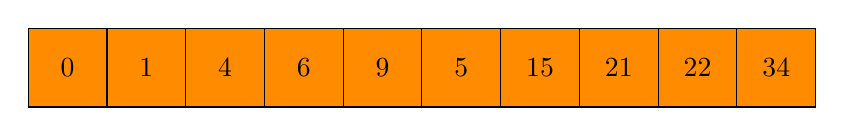
\begin{tikzpicture}
			\filldraw [draw=black, fill=tocheck] (0, 0) rectangle (1, 1) node[midway]{0};
			\filldraw [draw=black, fill=tocheck] (1, 0) rectangle (2, 1) node[midway]{1};
			\filldraw [draw=black, fill=tocheck] (2, 0) rectangle (3, 1) node[midway]{4};
			\filldraw [draw=black, fill=tocheck] (3, 0) rectangle (4, 1) node[midway]{6};
			\filldraw [draw=black, fill=tocheck] (4, 0) rectangle (5, 1) node[midway]{9};
			\filldraw [draw=black, fill=tocheck] (5, 0) rectangle (6, 1) node[midway]{5};
			\filldraw [draw=black, fill=tocheck] (6, 0) rectangle (7, 1) node[midway]{15};
			\filldraw [draw=black, fill=tocheck] (7, 0) rectangle (8, 1) node[midway]{21};
			\filldraw [draw=black, fill=tocheck] (8, 0) rectangle (9, 1) node[midway]{22};
			\filldraw [draw=black, fill=tocheck] (9, 0) rectangle (10, 1) node[midway]{34};
		\end{tikzpicture}
	\end{center}
	
	\noindent \\
	First we need to find the middle of our array. Our maximum index is 9 so half would be 4.5. Since only integers can be indices, let's round this to 4.
	\\
	So the element we are currently looking for has index 4 and to make it easier, let's call this the pivot element. In our array the pivot element has
	the value 9 (highlighted blue below).
	\begin{center}
		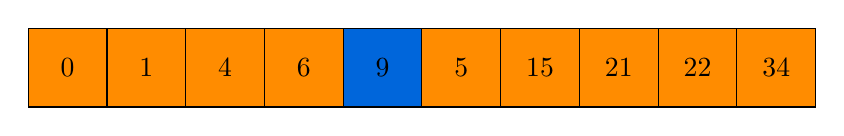
\begin{tikzpicture}
			\filldraw [draw=black, fill=tocheck] (0, 0) rectangle (1, 1) node[midway]{0};
			\filldraw [draw=black, fill=tocheck] (1, 0) rectangle (2, 1) node[midway]{1};
			\filldraw [draw=black, fill=tocheck] (2, 0) rectangle (3, 1) node[midway]{4};
			\filldraw [draw=black, fill=tocheck] (3, 0) rectangle (4, 1) node[midway]{6};
			\filldraw [draw=black, fill=currentfocus] (4, 0) rectangle (5, 1) node[midway]{9};
			\filldraw [draw=black, fill=tocheck] (5, 0) rectangle (6, 1) node[midway]{5};
			\filldraw [draw=black, fill=tocheck] (6, 0) rectangle (7, 1) node[midway]{15};
			\filldraw [draw=black, fill=tocheck] (7, 0) rectangle (8, 1) node[midway]{21};
			\filldraw [draw=black, fill=tocheck] (8, 0) rectangle (9, 1) node[midway]{22};
			\filldraw [draw=black, fill=tocheck] (9, 0) rectangle (10, 1) node[midway]{34};
		\end{tikzpicture}
	\end{center}
	\noindent \\
	Our pivot is no equals to 21, so we haven't reached our goal yet. But since the list is sorted and 9 is less than 21, we know that both the pivot and
	everything on it's right side can not contain 21.
	\\
	This reduces the amount of elements we need to care about from 10 to 5.
	\begin{center}
		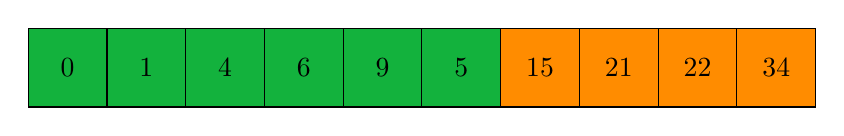
\begin{tikzpicture}
			\filldraw [draw=black, fill=checked] (0, 0) rectangle (1, 1) node[midway]{0};
			\filldraw [draw=black, fill=checked] (1, 0) rectangle (2, 1) node[midway]{1};
			\filldraw [draw=black, fill=checked] (2, 0) rectangle (3, 1) node[midway]{4};
			\filldraw [draw=black, fill=checked] (3, 0) rectangle (4, 1) node[midway]{6};
			\filldraw [draw=black, fill=checked] (4, 0) rectangle (5, 1) node[midway]{9};
			\filldraw [draw=black, fill=checked] (5, 0) rectangle (6, 1) node[midway]{5};
			\filldraw [draw=black, fill=tocheck] (6, 0) rectangle (7, 1) node[midway]{15};
			\filldraw [draw=black, fill=tocheck] (7, 0) rectangle (8, 1) node[midway]{21};
			\filldraw [draw=black, fill=tocheck] (8, 0) rectangle (9, 1) node[midway]{22};
			\filldraw [draw=black, fill=tocheck] (9, 0) rectangle (10, 1) node[midway]{34};
		\end{tikzpicture}
	\end{center}
	Sep
	\begin{center}
		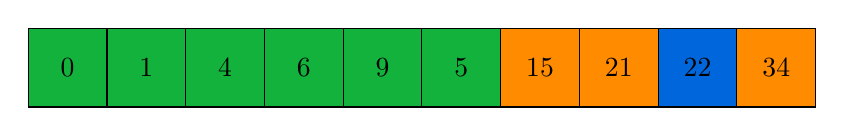
\begin{tikzpicture}
			\filldraw [draw=black, fill=checked] (0, 0) rectangle (1, 1) node[midway]{0};
			\filldraw [draw=black, fill=checked] (1, 0) rectangle (2, 1) node[midway]{1};
			\filldraw [draw=black, fill=checked] (2, 0) rectangle (3, 1) node[midway]{4};
			\filldraw [draw=black, fill=checked] (3, 0) rectangle (4, 1) node[midway]{6};
			\filldraw [draw=black, fill=checked] (4, 0) rectangle (5, 1) node[midway]{9};
			\filldraw [draw=black, fill=checked] (5, 0) rectangle (6, 1) node[midway]{5};
			\filldraw [draw=black, fill=tocheck] (6, 0) rectangle (7, 1) node[midway]{15};
			\filldraw [draw=black, fill=tocheck] (7, 0) rectangle (8, 1) node[midway]{21};
			\filldraw [draw=black, fill=currentfocus] (8, 0) rectangle (9, 1) node[midway]{22};
			\filldraw [draw=black, fill=tocheck] (9, 0) rectangle (10, 1) node[midway]{34};
		\end{tikzpicture}
	\end{center}
	\begin{center}
		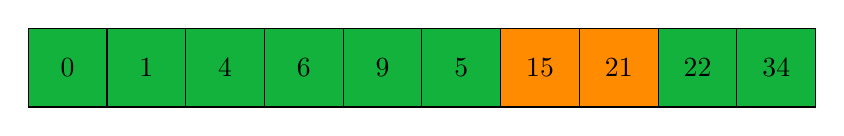
\begin{tikzpicture}
			\filldraw [draw=black, fill=checked] (0, 0) rectangle (1, 1) node[midway]{0};
			\filldraw [draw=black, fill=checked] (1, 0) rectangle (2, 1) node[midway]{1};
			\filldraw [draw=black, fill=checked] (2, 0) rectangle (3, 1) node[midway]{4};
			\filldraw [draw=black, fill=checked] (3, 0) rectangle (4, 1) node[midway]{6};
			\filldraw [draw=black, fill=checked] (4, 0) rectangle (5, 1) node[midway]{9};
			\filldraw [draw=black, fill=checked] (5, 0) rectangle (6, 1) node[midway]{5};
			\filldraw [draw=black, fill=tocheck] (6, 0) rectangle (7, 1) node[midway]{15};
			\filldraw [draw=black, fill=tocheck] (7, 0) rectangle (8, 1) node[midway]{21};
			\filldraw [draw=black, fill=checked] (8, 0) rectangle (9, 1) node[midway]{22};
			\filldraw [draw=black, fill=checked] (9, 0) rectangle (10, 1) node[midway]{34};
		\end{tikzpicture}
	\end{center}
	Sep
	\begin{center}
		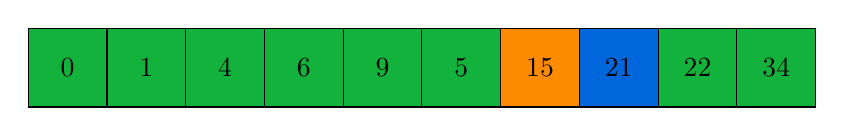
\begin{tikzpicture}
			\filldraw [draw=black, fill=checked] (0, 0) rectangle (1, 1) node[midway]{0};
			\filldraw [draw=black, fill=checked] (1, 0) rectangle (2, 1) node[midway]{1};
			\filldraw [draw=black, fill=checked] (2, 0) rectangle (3, 1) node[midway]{4};
			\filldraw [draw=black, fill=checked] (3, 0) rectangle (4, 1) node[midway]{6};
			\filldraw [draw=black, fill=checked] (4, 0) rectangle (5, 1) node[midway]{9};
			\filldraw [draw=black, fill=checked] (5, 0) rectangle (6, 1) node[midway]{5};
			\filldraw [draw=black, fill=tocheck] (6, 0) rectangle (7, 1) node[midway]{15};
			\filldraw [draw=black, fill=currentfocus] (7, 0) rectangle (8, 1) node[midway]{21};
			\filldraw [draw=black, fill=checked] (8, 0) rectangle (9, 1) node[midway]{22};
			\filldraw [draw=black, fill=checked] (9, 0) rectangle (10, 1) node[midway]{34};
		\end{tikzpicture}
	\end{center}
\end{document}